\documentclass[titlepage]{article}

\usepackage[norsk]{babel}
\usepackage[T1]{fontenc}
\usepackage[utf8]{inputenc}

\usepackage{graphicx}
\usepackage{float}
\usepackage{url}
\usepackage{subfig}
\usepackage{listings}
\usepackage{verbatim}
\usepackage{SIunits}
\usepackage{multirow}
\usepackage{subfig}
\usepackage{hyperref}
\usepackage[hmargin=2cm,vmargin=2.5cm]{geometry}
\usepackage{listings}

\newcommand{\HRule}{\rule{\linewidth}{0.5mm}}
\usepackage[parfill]{parskip}

\begin{document}
%-----------------------------------------------------------
\begin{titlepage}
 
\begin{center}
 
\textsc{\LARGE TDT4225 Store Datamengder}\\[1.5cm]
\textsc{\Large Øving 1}\\[0.5cm]
 
\HRule \\[0.4cm]
{ \huge \bfseries Test av lesehastigheter}\\[0.4cm]
\HRule \\[1.5cm]

Trond Klakken \\
Elisabeth Solheim \\
Gunnar Inge Gjøvik Sortland

\vfill
 
% Bottom of the page
{\large \today}
 
\end{center}

\end{titlepage}

\section{Oppsett}
Vi har i dette forsøket målt lesetid for en fil på 1GB fra tre ulike
lagringsmedier.

Disse var Solid State disk (SSD) (\ref{SSD}), USB-minnepinne
(\ref{USB}) og fra ordinær disk (\ref{HDD}). For å sikre at hver test
ble uavhengig ble en fil på 1GB lest inn mellom hver av de, for å
flushe cache.

Testprogrammet kjører automatisk benchmarking for de 21 test
tilfellende gitt av oppgaven, og ble kjørt på hver av de tre mediene.

Grunnet mangel på tilgjengelig utstyr ble testene kjørt på to ulike
maskiner. Spesifikasjoner er gitt i tabell \ref{tab:hardware}. Dette
kan medføre at ulikheter i lesehastighet ikke bare skyldes mediet, men
også andre forhold. Trendene vi ser bør likevel være representive.

\begin{table}[h!]
 \caption{Benyttet maskinvare}
 \label{tab:hardware}
  \centering
  \begin{tabular}{|l|l|l|l|l|}
\hline
\textbf{Lagringsmedium} & \textbf{OS} & Filsystem  & Disk & Hardware \\
\hline
\hline
SSD & OSX    & HFS+  & 550 mbps & MacBook Pro 15" \\
USB & OSX    & FAT32 & 8mbps    &MacBook Pro 15" med USB 2.1 \\
HDD & Ubuntu & ext4  & 7200 rpm SATA (120 GB) & Intel Core2 CPU 2.13 GHz \\

\hline
\end{tabular}
\end{table}

\section{Forventninger}
Vi forventer en graf der større blokkstørrelse gir raskere
resultater. Det er også forventet at jo flere filer som blir lest
samtidlig, jo dårligere blir ytelsen. Dette fordi de forskjellige
filene vil avbryte hverandre med interupts.  På random forventer vi
gjevnt dårlige resultater, siden den må hoppe såpass mye.

 SSD forventes å være raskest og best på random, siden den har det
 enklere å hoppe enn harddisken som må flytte leserhodet. USBen er
 forventet å oppføre seg mye som SDD-en, bare tregere.

Den optimale blokkstørrelsen ville være en som fylter opp
minnebåndbredden, slik at du ikke har tomme spor, eller må dele opp
blokkene i flere mindre blokker med tomme spor.

Vi forventer en del forstyrrelser fra OS, men regner med at SSD vil
være raskest, så HDD og til slutt USB.


\section{Resultater}

\begin{comment}
\begin{table}%[h!]
\caption{Lesing av fil fra SSD OS (OSX)}
\label{SSD}
\centering
\begin{tabular}{|l|l|l|l|}
\hline
\multirow{2}{*}{ Antall parallelle delfiler} & \multicolumn{3}{|c|}{Blokkstørrelse} \\
 & 1024 & 4096 & 16384\\
\hline
1         &  0.211783  &  0.077320  & 0.048120 \\
2         &  0.214290  &  0.080882  & 0.049755 \\
4         &  9.423701  &  9.105014  & 1.996882 \\
8         & 11.315957  & 10.991903  & 3.694221 \\
16        & 11.201126  &  0.088839  & 0.054831 \\
32        &  6.082929  &  4.833985  & 1.345019 \\
tilfeldig &  0.557162  &  0.528545  & 0.455504 \\
\hline
\end{tabular}
\end{table}

\begin{figure}%[h!]
  \caption{SSD}
  \label{fig:sdd}
  \centering
  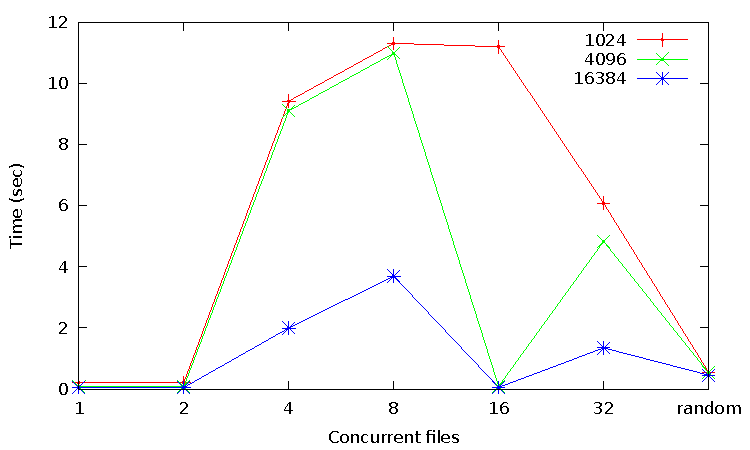
\includegraphics[width=0.5\textwidth]{res/result-sdd}
\end{figure}
\end{comment}

\begin{table}%[h!]
\caption{Lesing av fil fra USB minnepenn OS (OSX)}
\label{USB}
\centering
\begin{tabular}{|l|l|l|l|}
\hline
\multirow{2}{*}{ Antall parallelle delfiler} & \multicolumn{3}{|c|}{Blokkstørrelse} \\
 & 1024 & 4096 & 16384\\
\hline
1         & 44.858 & 44.847 & 44.863\\
2         & 44.978 & 44.929 & 44.995\\
4         & 44.929 & 44.926 & 44.975\\
8         & 44.950 & 44.958 & 45.018\\
16        & 44.964 & 44.962 & 44.973\\
32        & 44.906 & 44.911 & 45.061\\
\hline
\end{tabular}
\end{table}

\begin{figure}%[h!]
  \caption{Plot of reading times using USB stick}
  \label{fig:usb}
  \centering
  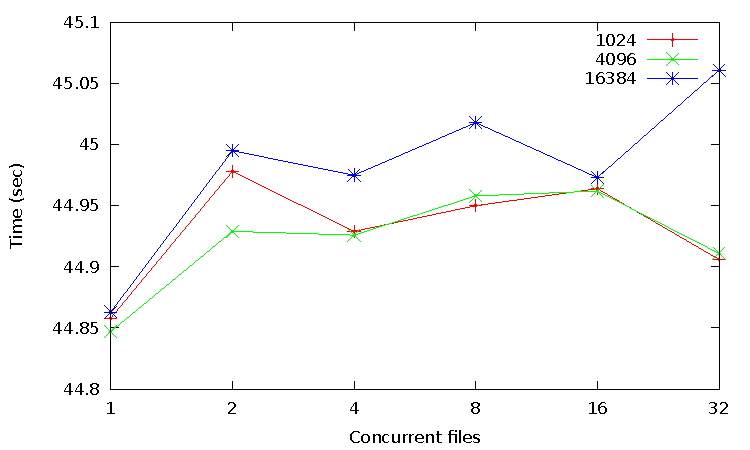
\includegraphics[width=0.5\textwidth]{res/result-usb}
\end{figure}

\begin{table}%[h!]
\caption{Lesing av fil fra magnetisk harddisk (Linux)}
\label{HDD}
\centering
\begin{tabular}{|l|l|l|l|}
\hline
\multirow{2}{*}{ Antall parallelle delfiler} & \multicolumn{3}{|c|}{Blokkstørrelse} \\
 & 1024 & 4096 & 16384\\
\hline
1         & 18.377  & 18.435 & 21.025 \\
2         & 32.766  & 32.499 & 33.107 \\
4         & 30.182  & 33.636 & 29.457 \\
8         & 33.599  & 30.309 & 29.408 \\
16        & 41.574  & 51.789 & 44.238 \\
32        & 63.257  & 64.565 & 80.174 \\
tilfeldig & 606.419 &        &        \\
\hline
\end{tabular}
\end{table}

\begin{figure}%[h!]
  \caption{HDD}
  \label{fig:hdd}
  \centering
  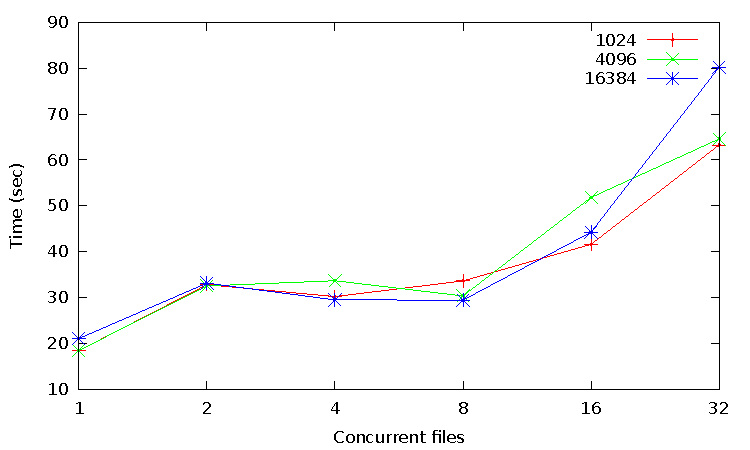
\includegraphics[width=0.5\textwidth]{res/result-hdd}
\end{figure}

\begin{comment}
Tabell \ref{SSD} og figur \ref{fig:sdd} viser kjøring ved SSD. Vi ser
en generell trend ved at økt blokkstørrelse gir lavere lesetid. Ved
økt antall parallelle åpne filer får vi noe høyere lesetid.
\end{comment}

Slik tabell \ref{USB} og figur \ref{fig:usb} viser påvirkes ikke
lesing fra USB av uregelmessig aksessmønster ved flere åpne filer. Vi
rakk desverre ikke å få kjørt denne med test av tilfeldig lesing.

\begin{figure}%[h!]
  \centering
  \subfloat[1024]{\label{fig:1024}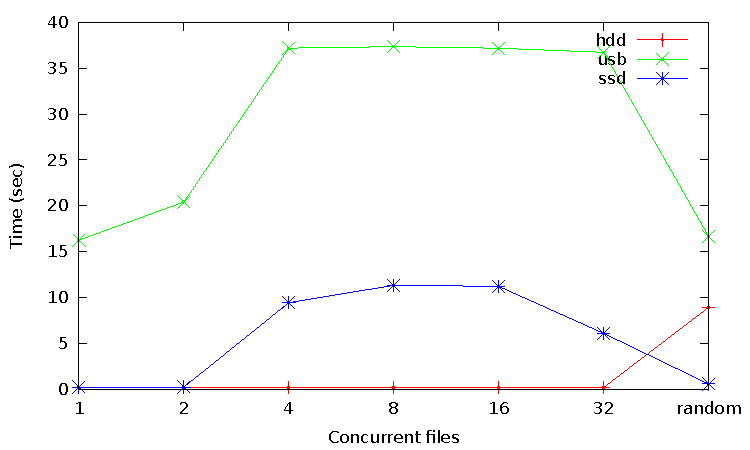
\includegraphics[width=0.3\textwidth]{res/1024}}
  \subfloat[4096]{\label{fig:4096}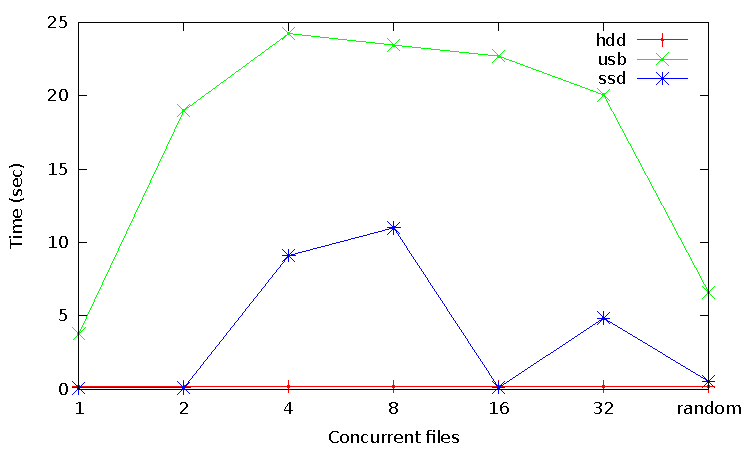
\includegraphics[width=0.3\textwidth]{res/4096}}
  \subfloat[16386]{\label{fig:16386}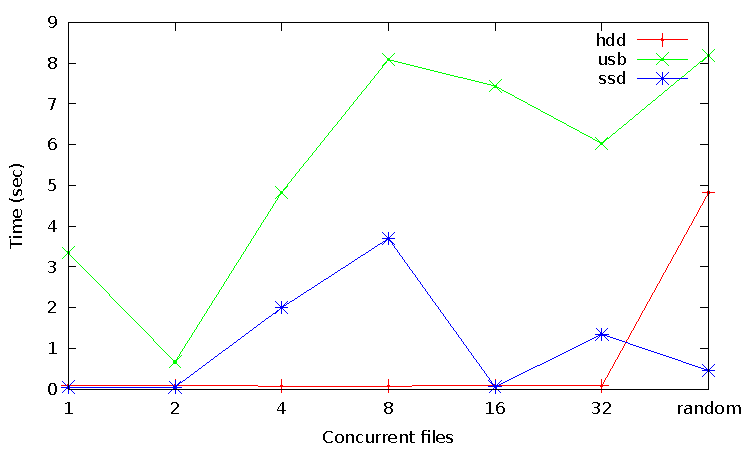
\includegraphics[width=0.3\textwidth]{res/16386}}
  \caption{Lesetid for hvert medium ved ulike blokkstørrelser}
  \label{fig:blocksizes}
\end{figure}

Figur \ref{fig:blocksizes} sammenligner lesehastighet ved hver av
gitte blokkstørrelsene.

\section{Drøfting og konklusjon}
Grunnet en feil i koden, ble resultatene noe feil. Vi har kjørt ny test på magnetisk
disk, slik at disse resultatene skal være korrekte.

Ved bruk av SSD er søketiden relativt lav, slik at vi forventer at
dette ikke utgjør så mye som ved vanlig harddisk. Tabell \ref{HDD} og
figur \ref{fig:hdd} viser at dette ikke utgjør så mye som vi kunne
forvente.  På grunn av praktiske hensyn er det vanskelig å sammenligne
lesetid direkte, men trendene kan likevel sammenlignes.

Lesing via USB var, som nevnt, meget tregt.  Dette skyldes trolig at
overføringen er via USB og minnepennen var av billig modell.

Vi ser her at fra 4 til 32 parallelle filer påvirkes ikke
lesehastighet signifikant. Vi ser også her at større blokker gir
raskere lesing.

Lesing fra ordinær harddisk ble lite påvirket av blokkstørrelse. 
Vi ser derimot at flere parallele lesinger gir høyere lesetid, noe som skyldes
flere hopp.



\clearpage
\section{Appendix}

\clearpage
\subsection{\texttt{test.cpp} - Main program}
\lstinputlisting{../code/test.cpp}

\subsection{\texttt{Makefile}}
\lstinputlisting{../code/Makefile}

\clearpage
\subsection{\texttt{benchmark.h}}
\lstinputlisting{../code/benchmark.h}

\clearpage
\subsection{\texttt{benchmark.cpp}}
\lstinputlisting{../code/benchmark.cpp}

\end{document}
